\section{Automatic Stream Management Using Program Contexts}

In developing \textsf{\small PCStream}, our key insight was that in most applications,
(regardless of their I/O workload characteristics)
a few dominant I/O activities exist
and each dominant I/O activity   
represents the application's important I/O context (e.g., for logging or for flushing). 
Furthermore, most dominant I/O activities tend to have distinct data lifetime patterns.
In order to distinguish data by their lifetimes, therefore, 
it is important to effectively distinguish dominant I/O activities from each other.  
For example, in update workloads, 
LBAs alone were effective in separating dominant I/O activities.  

In this paper, we argue that a program context is an efficient general-purpose
indicator for separating dominant I/O activities regardless of the type of I/O
workloads.  Since a PC represents an execution path of an application which
invokes write-related system functions such as {\tt write()} and {\tt writev()}
in the Linux kernel,  we represent the PC by summing program counter values of
all the functions along the execution path which leads to a write system call.

\subsection{Distinct Data Lifetime Patterns of Different PCs}
In order to show PCs are effective to distinguish I/O activities of
an application, we measured the lifetime distribution of different PCs for various
types of workloads.

In RocksDB, for example, dominant I/O activities include logging, flushing and
compaction.  Since they are invoked through different function-call paths, we
can easily identify dominant I/O activities of RocksDB using PCs.  For example,
Fig.~\ref{fig:getpc}(a) shows an execution path for flushing in RocksDB.  The
sum of program counter values of \texttt{Run()}, \texttt{WriteLevel0Table()},
and \texttt{BuildTable()} is used to represent the PC for the flushing
activity. Note that using the program context to distinguish data lifetimes is
not new. For example, Ha {\it et al.} proposed a data separation technique
based on the program context~\cite{PCHa}.  However, their work was neither
designed for append-only workloads nor for modern multi-streamed SSDs.

\begin{figure}[t]
\centering
\hfill
%\vspace{-10pt}
	\subfloat[Logging (PC)]{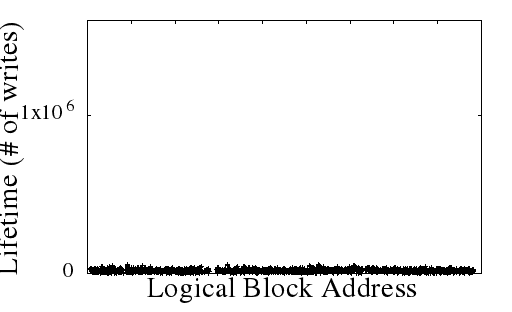
\includegraphics[width=0.2\textwidth]{figure/type_1}} % data from 4/03031953 
	\hspace{2pt}
	\subfloat[Logging (manual)]{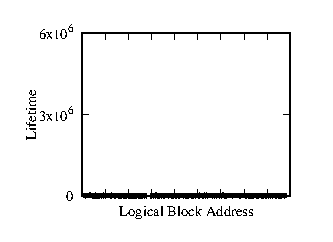
\includegraphics[width=0.2\textwidth]{figure/pcID_2}}
\hfill
\vspace{7pt}
	\subfloat[Flushing (PC)] {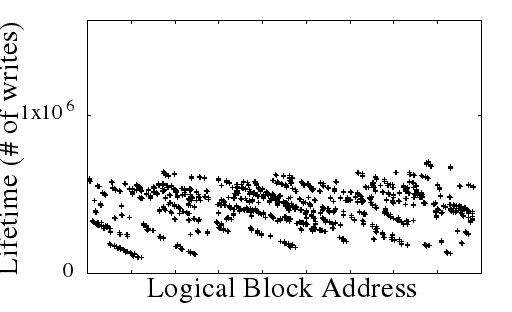
\includegraphics[width=0.2\textwidth]{figure/type_3}}
	\hspace{2pt}
	\subfloat[Flushing (manual)]{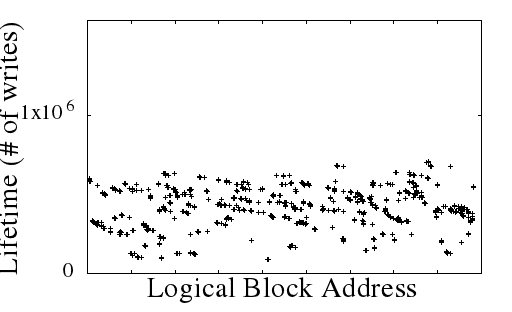
\includegraphics[width=0.2\textwidth]{figure/pcID_3}}
%\vspace{-7pt}
\caption{Data lifetime distributions of different PCs for an append-only workload.} 
\label{fig:types_and_PCs}
%\vspace{-20pt}
\end{figure}

In order to validate our hypothesis that PCs can be useful for predicting
lifetimes by distinguishing dominant I/O activities, we conducted experiments
using RocksDB, comparing the accuracy of identifying dominant I/O activities
using two different methods.  First, we manually identified dominant I/O
activities by inspecting the source code. Second, we automatically decided
dominant I/O activities by extracting PCs for write-related system functions.
Fig.~\ref{fig:types_and_PCs} illustrates two dominant I/O activities matched
between two methods.   As shown in Fig.~\ref{fig:types_and_PCs}(a)
and~\ref{fig:types_and_PCs}(b), the logging activity of RocksDB is correctly
identified by two methods.  Furthermore, from the logging-activity PC, we can
clearly observe that data written from the PC are short-lived. Similarly,
from Fig.~\ref{fig:types_and_PCs}(c) and~\ref{fig:types_and_PCs}(d), we observe
that data written from the flushing-activity PC behave in a different fashion.
For example, data from the flushing-activity PC remain valid a lot longer than
those from the logging-activity PC.

Furthermore, PCs are also effective for non-append-only workloads
in distinguishing I/O activities. 
In order to show the effect of PCperformed experiments ...
{\color{red} TODO: 추가 그림에 대한 설명 \\ \\ \\ \\ \\ \\ \\}
\begin{figure}[t]
\centering
\hfill
%\vspace{-10pt}
	\subfloat[sqlite (PC)]{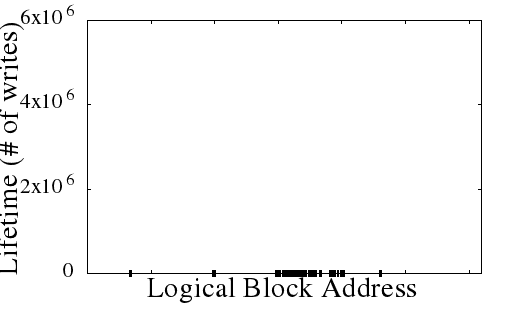
\includegraphics[width=0.2\textwidth]{figure/sqlite_short_LBA}} % data from py-tpcc/4/09151534
	\hspace{2pt}
	\subfloat[sqlite (manual)]{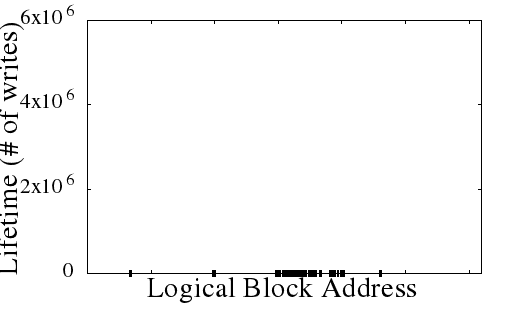
\includegraphics[width=0.2\textwidth]{figure/sqlite_short_LBA_manual}}
\hfill
\vspace{7pt}
	\subfloat[gcc (PC)] {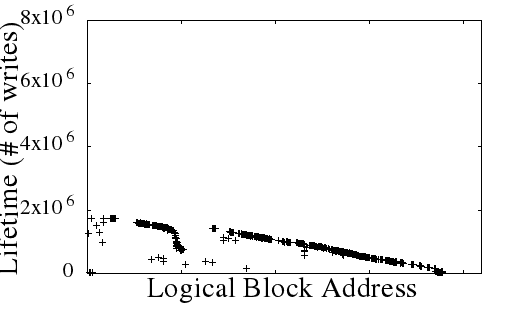
\includegraphics[width=0.2\textwidth]{figure/compile_short_PC}} % data from 08231319
	\hspace{2pt}
	\subfloat[gcc (manual)]{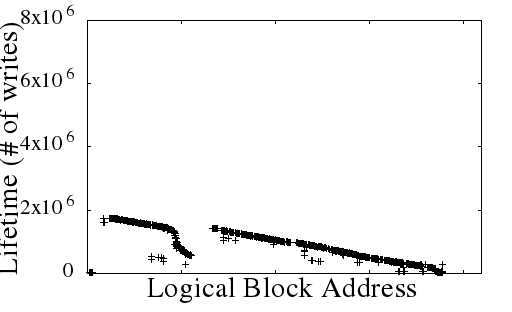
\includegraphics[width=0.2\textwidth]{figure/compile_short_manual}}
%\vspace{-7pt}
\caption{Data lifetime distributions of different PCs for updating workloads.} 
\label{fig:types_and_PCs}
%\vspace{-20pt}
\end{figure}


\subsection{Extracting PCs}
As mentioned earlier, a PC signature is defined to be the sum of program counter
values along the execution path of function calls that finally reaches a
write-related system function.  
In theory, program counter values in the
execution path can be extracted in a relatively straightforward manner.  Except
for inline functions, every function call involves pushing the address of the
next instruction of a caller as a return address to the stack, followed by
pushing a frame pointer value.  In general, by referring to frame pointer
values, we are able to back-track stack frames of a process and selectively get
return addresses for generating a PC signature.  For example,
Fig.~\ref{fig:getpc}(a) shows an abstracted execution path of flushing data in
RocksDB, and Fig.~\ref{fig:getpc}(b) illustrates how a PC signature is obtained
by back-tracking the stack.  The return addresses are pushed before calling the
\textsf{\small  write()}, \textsf{\small  BuildTable()} and \textsf{\small
WriteLevel0Table()} functions.  Since frame pointer values in the stack hold
the addresses of previous frame pointers, we can easily obtain return addresses
and accumulate them to compute a PC signature.  

The frame pointer-based approach for computing a PC signature, however, is not
always possible because modern C/C++ compilers often do not use a frame pointer
for improving the efficiency of register allocation.  One example is a {\tt
-fomit-frame-pointer} option of GCC~\cite{GCC}.  This option allows the frame
pointer to be used as a general-purpose register, but makes it difficult for us
to back-track return addresses along the call chains.  

\begin{figure}[t]
%	\vspace{-10pt}
	\centering
	%\vspace{-8pt}
	\subfloat[An abstracted execution path for flushing data.]{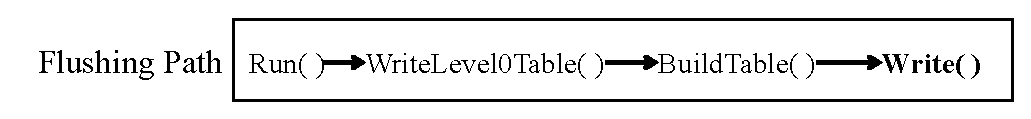
\includegraphics[width=0.4\textwidth]{figure/getpc_1}}  
	%\vspace{-14pt}
	\hfill
	\subfloat[with the frame pointer.]{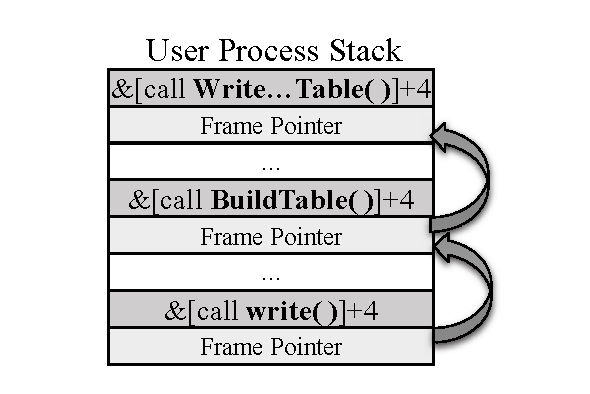
\includegraphics[width=0.22\textwidth]{figure/getpc_2}}
	\subfloat[without the frame pointer.]{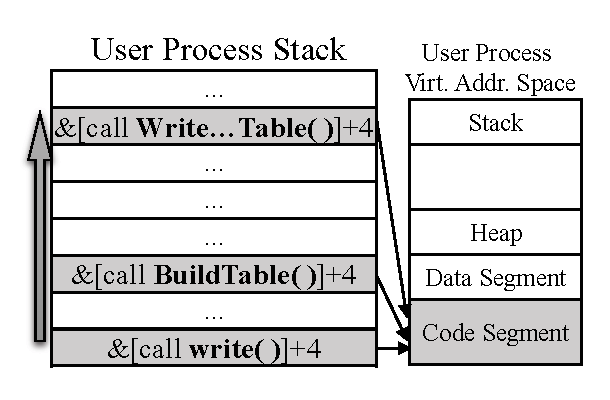
\includegraphics[width=0.22\textwidth]{figure/getpc_3}}
	%\vspace{-9pt}
	\caption{An example execution path and its PC extraction methods.}
	%\caption{An example execution path and its PC extraction.} %shane part
	\label{fig:getpc}
	%\vspace{-20pt}
\end{figure}

The PC extractor of \textsf{\small PCStream} employs a simple but effective
workaround for back-tracking a call stack when a frame pointer is not
available.  When a write system call is made, the PC extractor scans every word
in the stack and checks if it belongs to process's code segment.  If the
scanned stack word holds a value within the address range of the code segment,
it assumes that it is a return address.  Since scanning the entire stack takes
too long, we stop the scanning when a sufficient number of return address
candidates are found. In the current implementation, only five candidates are
used for PC computation.  Even though it is quite ad-hoc, this restricted scan
is effective in distinguishing different PCs; it is very unlikely that two
different PCs follow exactly the same execution path to the \textsf{\small
write()} system call.  In our evaluation with a 3.4 GHz CPU machine, the
overhead of the restricted scan was almost negligible, taking only 300-400
$n$sec per \textsf{\small write()} system call.





\subsection{Consistency of PCs across the execution}
Based on the fact that PCs are computed using the return addresses, 





